\begin{figure}[H]
\centering
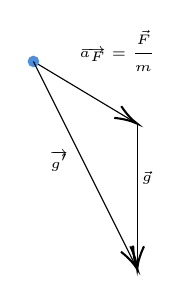
\begin{tikzpicture}[x=0.75pt,y=0.75pt,yscale=-1,xscale=1]
%uncomment if require: \path (0,300); %set diagram left start at 0, and has height of 300

%Straight Lines [id:da6000594042392968] 
\draw    (302.5,70) -- (350.79,98.97) ;
\draw [shift={(352.5,100)}, rotate = 210.96] [color={rgb, 255:red, 0; green, 0; blue, 0 }  ][line width=0.75]    (10.93,-3.29) .. controls (6.95,-1.4) and (3.31,-0.3) .. (0,0) .. controls (3.31,0.3) and (6.95,1.4) .. (10.93,3.29)   ;
%Shape: Circle [id:dp5092551209319207] 
\draw  [color={rgb, 255:red, 74; green, 144; blue, 226 }  ,draw opacity=1 ][fill={rgb, 255:red, 74; green, 144; blue, 226 }  ,fill opacity=1 ] (305,70) .. controls (305,68.62) and (303.88,67.5) .. (302.5,67.5) .. controls (301.12,67.5) and (300,68.62) .. (300,70) .. controls (300,71.38) and (301.12,72.5) .. (302.5,72.5) .. controls (303.88,72.5) and (305,71.38) .. (305,70) -- cycle ;
%Straight Lines [id:da48222497169597345] 
\draw    (352.5,100) -- (352.5,168) ;
\draw [shift={(352.5,170)}, rotate = 270] [color={rgb, 255:red, 0; green, 0; blue, 0 }  ][line width=0.75]    (10.93,-3.29) .. controls (6.95,-1.4) and (3.31,-0.3) .. (0,0) .. controls (3.31,0.3) and (6.95,1.4) .. (10.93,3.29)   ;
%Straight Lines [id:da2944838205191447] 
\draw    (302.5,70) -- (351.61,168.21) ;
\draw [shift={(352.5,170)}, rotate = 243.43] [color={rgb, 255:red, 0; green, 0; blue, 0 }  ][line width=0.75]    (10.93,-3.29) .. controls (6.95,-1.4) and (3.31,-0.3) .. (0,0) .. controls (3.31,0.3) and (6.95,1.4) .. (10.93,3.29)   ;

% Text Node
\draw (323.5,54) node [anchor=north west][inner sep=0.75pt]  [font=\tiny] [align=left] {$\displaystyle \overrightarrow{a_{F}} =\frac{\vec{F}}{m}$};
% Text Node
\draw (353.5,122) node [anchor=north west][inner sep=0.75pt]  [font=\tiny] [align=left] {$\displaystyle \vec{g}$};
% Text Node
\draw (309.5,112) node [anchor=north west][inner sep=0.75pt]  [font=\tiny] [align=left] {$\displaystyle \overrightarrow{g^{\prime }}$};


\end{tikzpicture}

\caption{受到恒力}
\end{figure}